\documentclass[xcolor={dvipsnames},aspectratio=169,10pt]{beamer}
\usetheme{mx}

\title{Finding a fETus with UltraSound (FETUS)}
\subtitle{King's Health Partners Summer School}
\author{
Shu Wang,
Ou Zhanchong, and
{\bf Miguel Xochicale}
}
\date{
King's Health Partners Summer School {\bf \#2021} \\
6th July 2021
}
\institute{
	\faEnvelope miguel.xochicale@kcl.ac.uk \\
	\faGithubAlt @mxochicale \faTwitter @\_mxochicale
		}
\githubrepository{https://github.com/xfetus/us-simulator}

\begin{document}

{
  \usebackgroundtemplate{\includegraphics[width=\paperwidth]{./figures/background-for-titlepage/versions/drawing-v00.png}}%
%    \usebackgroundtemplate{\includegraphics{./figures//image-for-title-background/versions/drawing-v00.png}}%
  \maketitle
}


\begin{frame}{Contents}
    \tableofcontents
\end{frame}

%%%%%%%%%%%%%%%%%%%%%%%%%%%%%%%%%%%%%%%%%%%%
\section{Who?, Why? Where?}


%%%%%%%%%%%%%%%%%%%%%%%%%%%%%%%%%%%%%%%%%%%%%
%\subsection{FETUS}

%%%%%%%%%%%%%%%%%%%%%%%%%%%%%%%%%%%%%%%%%%%%%%%%%%%%%%%%
{
%\paper{Lastname N. YEAR in journal of...}
\begin{frame}{Who am I?}

  \begin{figure}
  \centering
  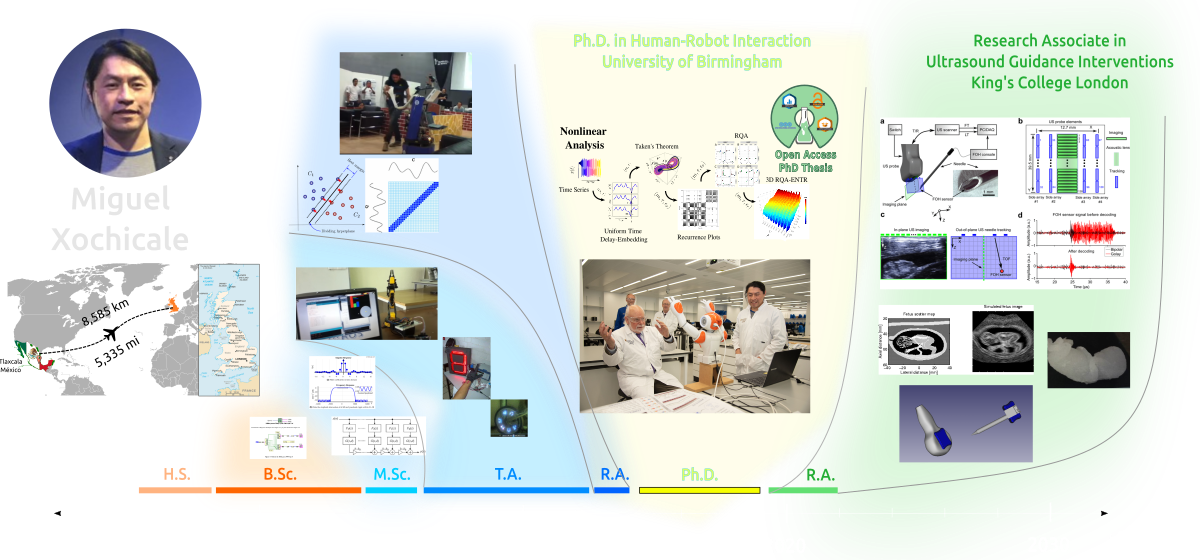
\includegraphics[width=1.0\textwidth]{./figures/miguel-xochicale/versions/drawing-v03.png}
  \end{figure}

\end{frame}
}


%%%%%%%%%%%%%%%%%%%%%%%%%%%%%%%%%%%%%%%%%%%%%
%\subsection{FETUS}

%%%%%%%%%%%%%%%%%%%%%%%%%%%%%%%%%%%%%%%%%%%%%%%%%%%%%%%%
{
%\paper{Lastname N. YEAR in journal of...}
\begin{frame}{Who are we? / Where we come from? / Do we have hobbies?}

  \begin{figure}
  \centering
  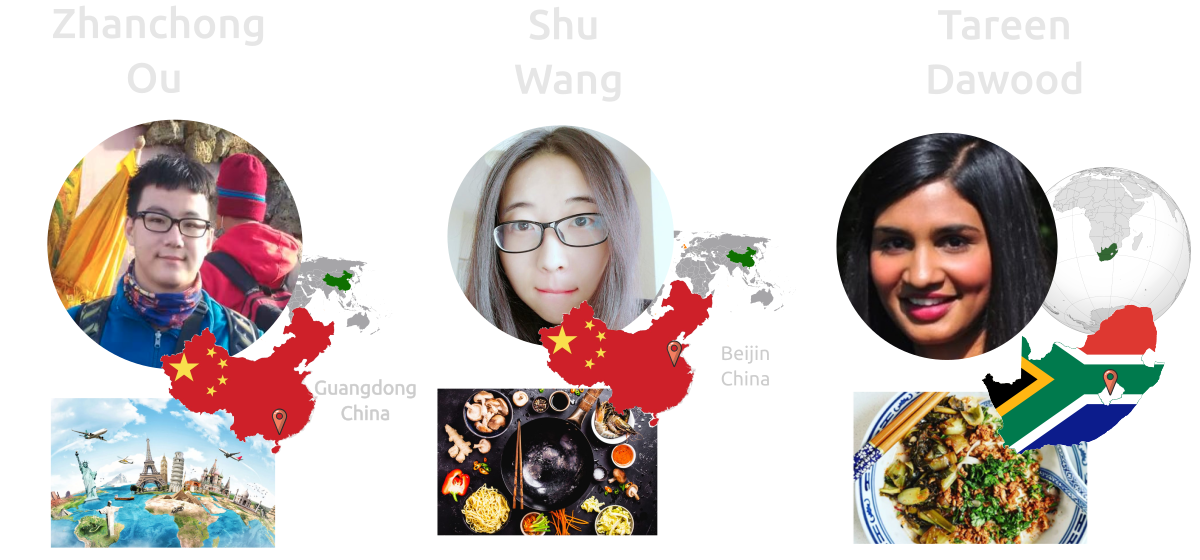
\includegraphics[width=1.0\textwidth]{./figures/who-we-are/versions/drawing-v06.png}
  \end{figure}

\end{frame}
}



%%%%%%%%%%%%%%%%%%%%%%%%%%%%%%%%%%%%%%%%%%%%%%%%%%%%%%%%
{
%\paper{}
\begin{frame}{}

\BigSizeFont
What does a Biomedical Engineer do?
\end{frame}
}



%%%%%%%%%%%%%%%%%%%%%%%%%%%%%%%%%%%%%%%%%%%%%
%\subsection{FETUS}

%%%%%%%%%%%%%%%%%%%%%%%%%%%%%%%%%%%%%%%%%%%%%%%%%%%%%%%%
{
%\paper{Lastname N. YEAR in journal of...}
\begin{frame}{}

  \begin{figure}
  \centering
  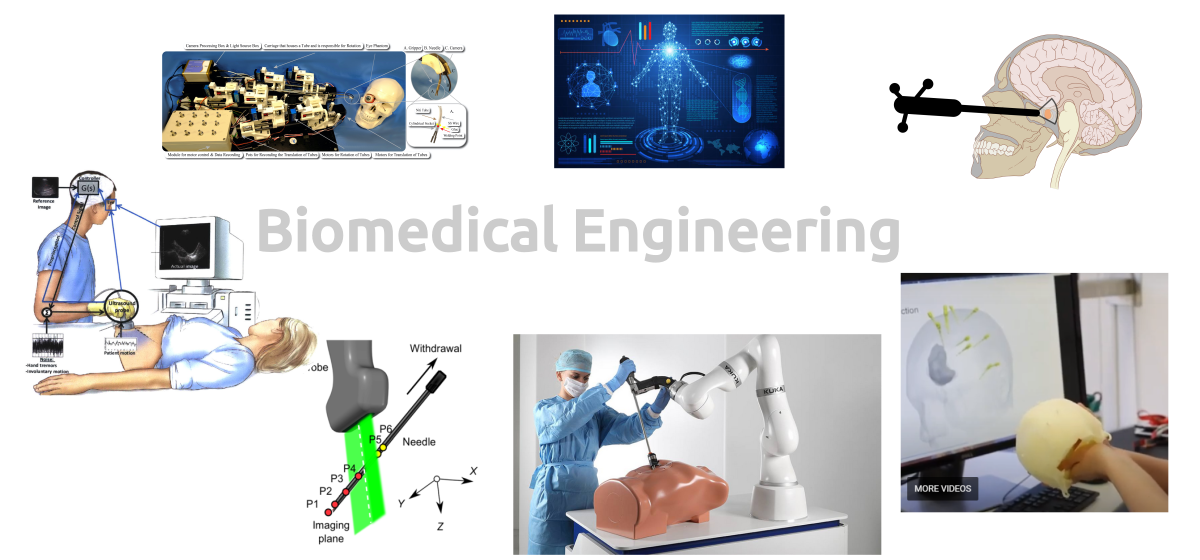
\includegraphics[width=1.0\textwidth]{./figures/biomedical-engineer/versions/drawing-v01.png}
  \end{figure}

\end{frame}
}



%%%%%%%%%%%%%%%%%%%%%%%%%%%%%%%%%%%%%%%%%%%%%
%\subsection{FETUS}

%%%%%%%%%%%%%%%%%%%%%%%%%%%%%%%%%%%%%%%%%%%%%%%%%%%%%%%%
{
%\paper{Lastname N. YEAR in journal of...}
\begin{frame}{Where we are based?}

  \begin{figure}
  \centering
  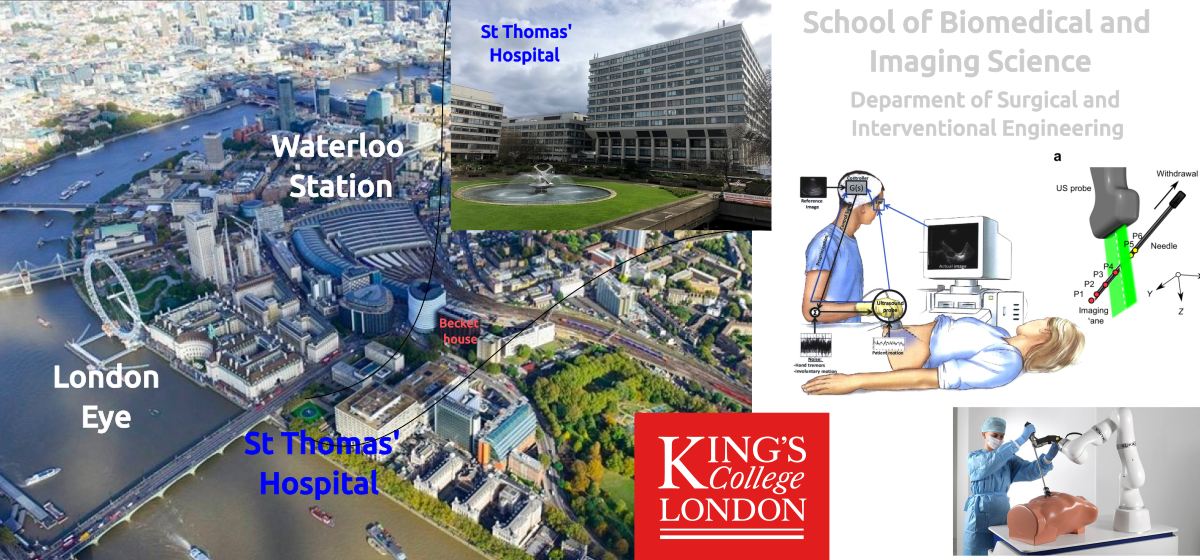
\includegraphics[width=1.0\textwidth]{./figures/where-we-are-based/versions/drawing-v02.png}
  \end{figure}

\end{frame}
}



%%%%%%%%%%%%%%%%%%%%%%%%%%%%%%%%%%%%%%%%%%%%%%%%%%%%%%%%
{
%\paper{}
\begin{frame}{}

\BigSizeFont
If you were a Sonographer for a day,
what do you think would be the most challenging activities you would encounter?

\end{frame}
}




%%%%%%%%%%%%%%%%%%%%%%%%%%%%%%%%%%%%%%%%%%%%
\section{Guessing Fetal Growth}

%%%%%%%%%%%%%%%%%%%%%%%%%%%%%%%%%%%%%%%%%%%%%
%\subsection{FETUS}


%%%%%%%%%%%%%%%%%%%%%%%%%%%%%%%%%%%%%%%%%%%%%%%%%%%%%%%%
{
\paper{Growing Baby: 3D Print-ready Models}
\begin{frame}{Fetal Growth}
      \begin{figure}
        \centering
        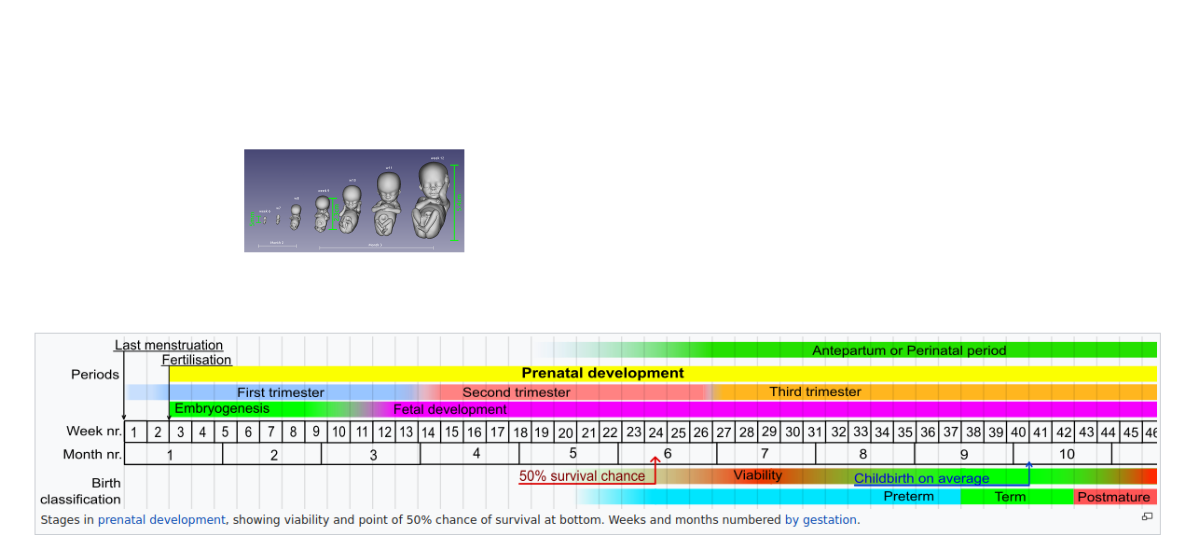
\includegraphics[width=1.0\textwidth]{./figures/fetal-growth/versions/drawing-v01.png}
        %\caption{}
      \end{figure}
\end{frame}
}


%%%%%%%%%%%%%%%%%%%%%%%%%%%%%%%%%%%%%%%%%%%%%%%%%%%%%%%%
{
\paper{Growing Baby: 3D Print-ready Models}
\begin{frame}{Fetal Growth}
      \begin{figure}
        \centering
        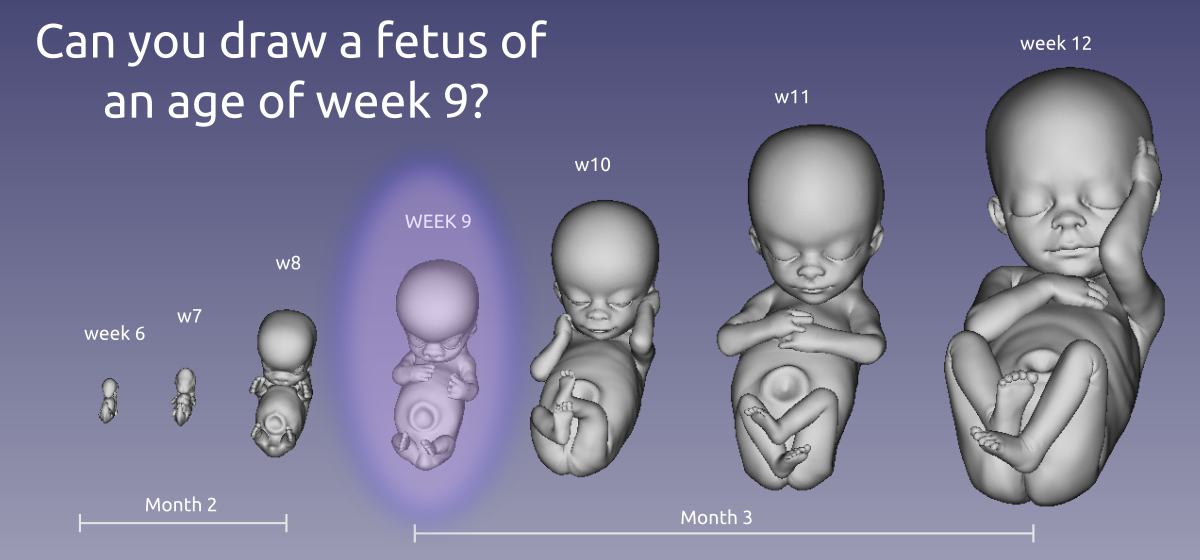
\includegraphics[width=1.0\textwidth]{./figures/fetal-growth/versions/drawing-v02.png}
        %\caption{}
      \end{figure}
\end{frame}
}







%%%%%%%%%%%%%%%%%%%%%%%%%%%%%%%%%%%%%%%%%%%%%%%%%%%%%%%%
{
\paper{ de Bakker et al. 2016 in Science \url{http://3datlas.3dembryo.nl/}; \url{https://www.whattoexpect.com/pregnancy/}}
\begin{frame}{Can you guess the *SIZE* of these fetus?}
      \begin{figure}
        \centering
        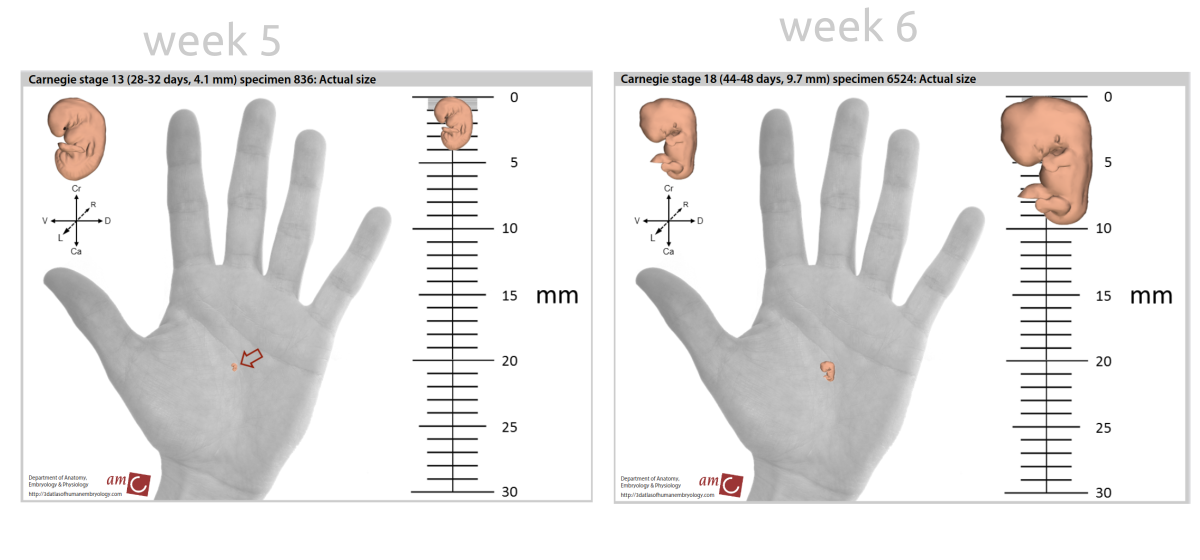
\includegraphics[width=1.0\textwidth]{./figures/fetal-size/versions/drawing-v01.png}
        %\caption{}
      \end{figure}
\end{frame}
}




%%%%%%%%%%%%%%%%%%%%%%%%%%%%%%%%%%%%%%%%%%%%%%%%%%%%%%%%
{
\paper{ de Bakker et al. 2016 in Science \url{http://3datlas.3dembryo.nl/}; \url{https://www.whattoexpect.com/pregnancy/}}
\begin{frame}{Can you guess the *SIZE* of these fetus?}
      \begin{figure}
        \centering
        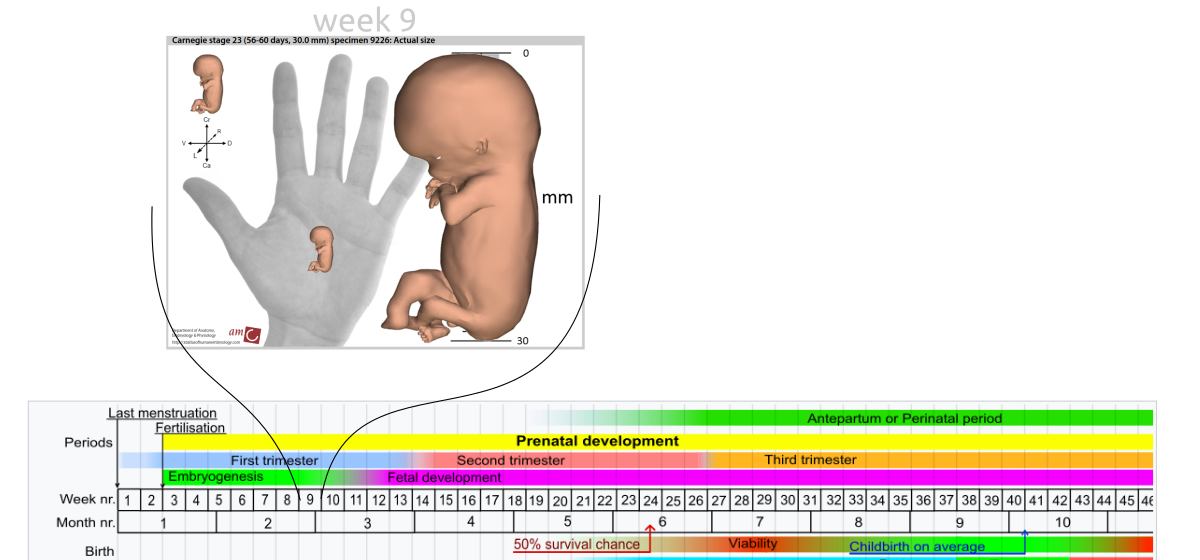
\includegraphics[width=1.0\textwidth]{./figures/fetal-size/versions/drawing-v02.png}
        %\caption{}
      \end{figure}
\end{frame}
}



%%%%%%%%%%%%%%%%%%%%%%%%%%%%%%%%%%%%%%%%%%%%
\section{Looking inside the human body}

%%%%%%%%%%%%%%%%%%%%%%%%%%%%%%%%%%%%%%%%%%%%%
%\subsection{FETUS}
%Medical imaging in pregnancy

%%%%%%%%%%%%%%%%%%%%%%%%%%%%%%%%%%%%%%%%%%%%%%%%%%%%%%%%
{
\paper{\url{https://en.wikipedia.org/wiki/Medical_imaging_in_pregnancy}}
\begin{frame}{Medical Imaging in Pregnancy}
      \begin{figure}
        \centering
        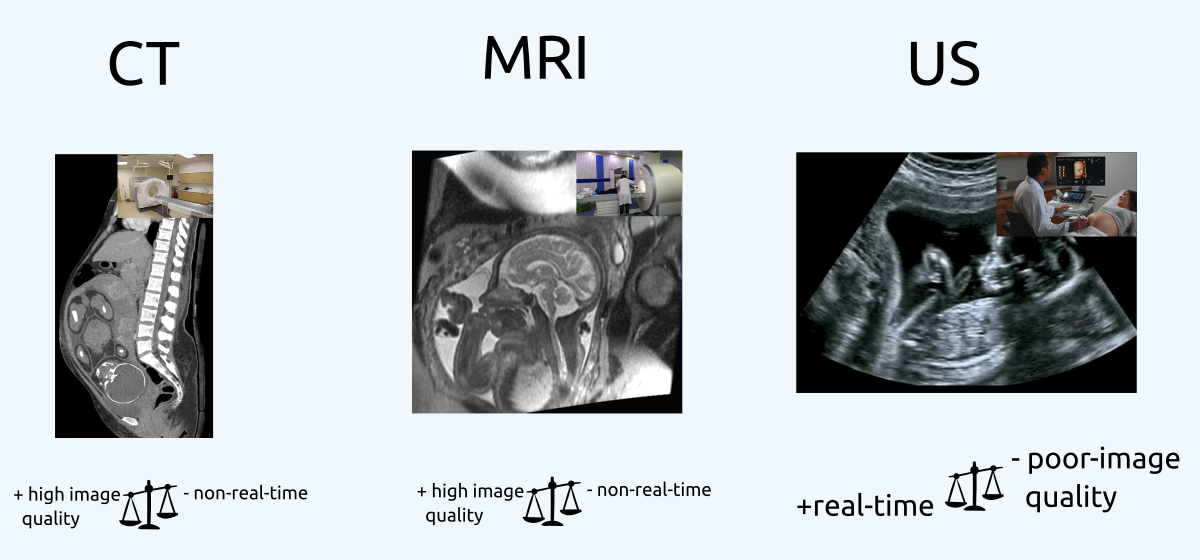
\includegraphics[width=1.0\textwidth]{./figures/medical-imaging/versions/drawing-v01.png}
        %\caption{}
      \end{figure}
\end{frame}
}


%%%%%%%%%%%%%%%%%%%%%%%%%%%%%%%%%%%%%%%%%%%%%%%%%%%%%%%%
{

\paper{Fetal and Mother Numerical Models (FEMONUM) in \url{http://femonum.telecom-paristech.fr}}
%https://perso.telecom-paristech.fr/angelini/projects_research/FEMONUM/femonum_en.html
%https://perso.telecom-paristech.fr/angelini/projects_research/FEMONUM/femonum_en.html

\begin{frame}{Modelling US imaging}
      \begin{figure}
        \centering
        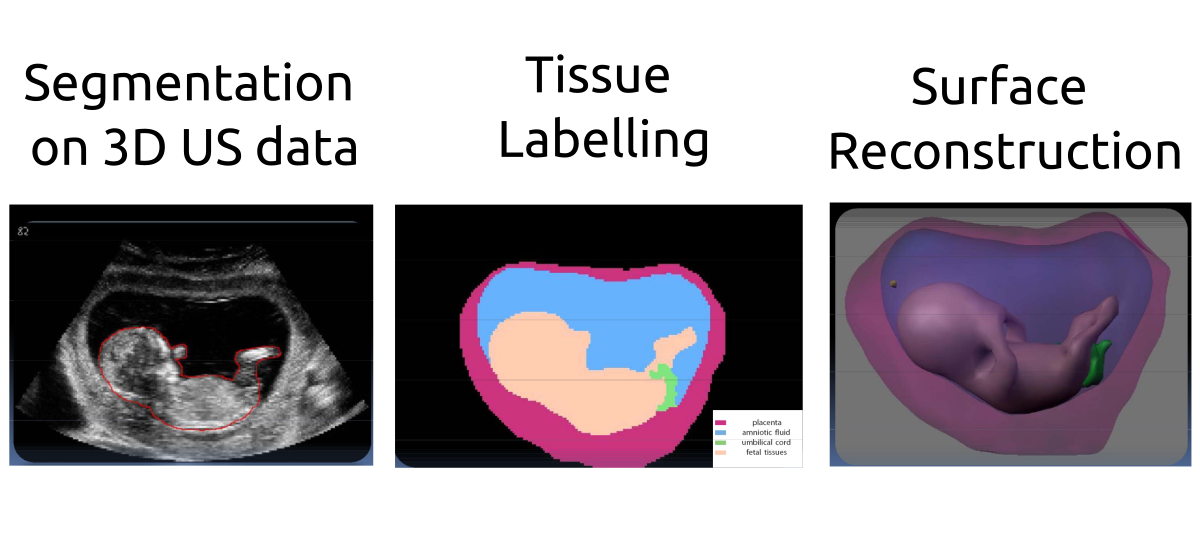
\includegraphics[width=1.0\textwidth]{./figures/modelling-us-imaging/versions/drawing-v01.png}
        %\caption{}
      \end{figure}
\end{frame}
}


%%%%%%%%%%%%%%%%%%%%%%%%%%%%%%%%%%%%%%%%%%%%%%%%%%%%%%%%
{
\paper{Add references}
\begin{frame}
  \frametitle{How to do and Why to do 3D printing?}
  \vspace{10pt}
        \begin{figure}
        \centering
        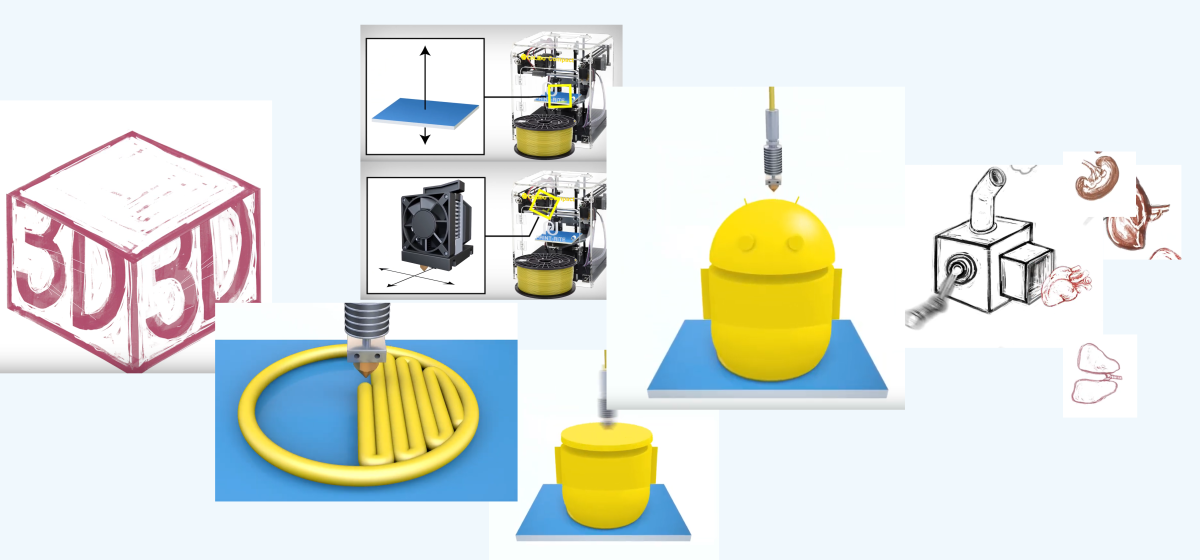
\includegraphics[width=1.0\textwidth]{./figures/3d-printing/why-and-how/versions/drawing-v00.png}
        %\caption{}
      \end{figure}

\end{frame}
}

%%%%%%%%%%%%%%%%%%%%%%%%%%%%%%%%%%%%%%%%%%%%%%%%%%%%%%%%
{
\paper{Add references}
\begin{frame}
  \frametitle{3D printing Fetus}
  \vspace{10pt}
  \begin{center}
    \movie{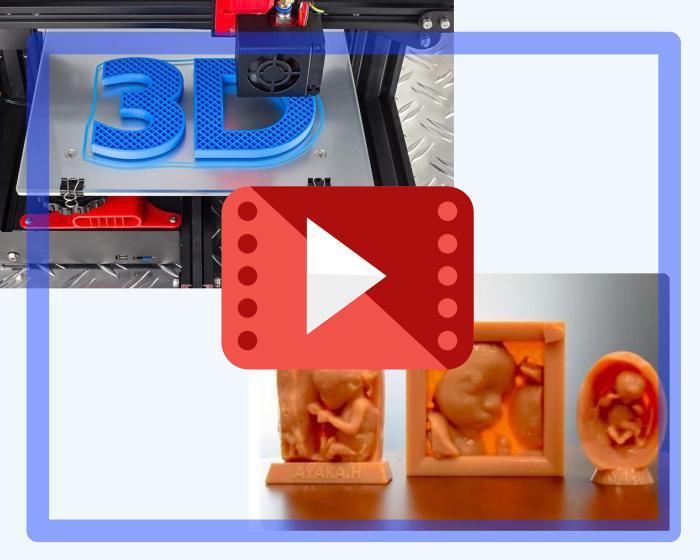
\includegraphics[width=0.5\textwidth]{./figures/3d-printing/video-of-printing-process/versions/drawing-v01.png}}{./figures/3d-printing/video-of-printing-process/videos/apollo17.avi}
  \end{center}
%  \begin{itemize}
%    \item Click on the image to play/pause the video.
%    \item Move pointer to the bottom of the video frame for a draggable position  control.
%  \end{itemize}
\end{frame}
}





%%%%%%%%%%%%%%%%%%%%%%%%%%%%%%%%%%%%%%%%%%%%
\section{Simulating Ultrasound-Guidance Interventions}


%%%%%%%%%%%%%%%%%%%%%%%%%%%%%%%%%%%%%%%%%%%%%%%%%%%%%%%%
{
\paper{Wright-Gilbertson M. 2014 in PhD thesis: Xia et al., 2017 in Scientific Reports}
\begin{frame}{The sonographer-probe-patient control system}
      \begin{figure}
        \centering
        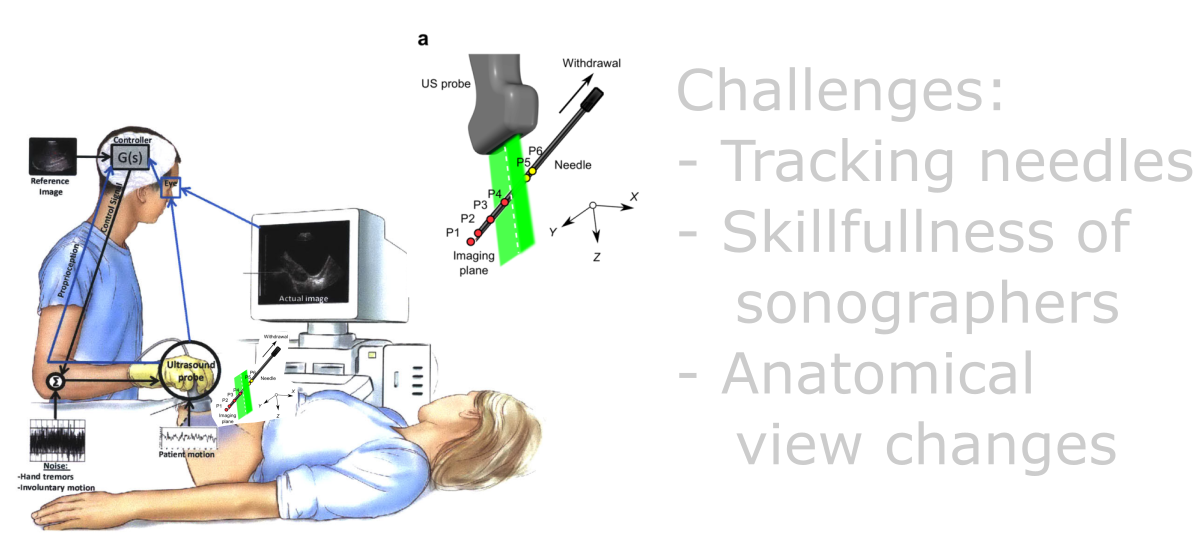
\includegraphics[width=1.0\textwidth]{./figures/sonographer-probe-patient/versions/drawing-v02.png}
        %\caption{}
      \end{figure}
\end{frame}
}





%%%%%%%%%%%%%%%%%%%%%%%%%%%%%%%%%%%%%%%%%%%%%%%%%%%%%%%%%
%{
%\paper{(a) Coordinate systems overview sketch in 3D Slicer,  (b) Asselin et al. 2018 in conf-BIVPCS, (c) US-simulator, and (d) 3D-printed fetus}
%\begin{frame}{Simulator for Ultrasound-Guidance Interventions}
%
%  \begin{columns}
%    \begin{column}{.3\linewidth}
%      Towards a more realistic
%  \begin{itemize}
%    \item \textbf{UGI}
%    \item \textbf{US images}
%    \item \textbf{Phantoms with 3D-printed US compatible material}
%    \item \textbf{Training for in-plane, out-of-plane needle tracking}
%  \end{itemize}
%
%    \end{column}
%
%
%  \begin{column}{.6\linewidth}
%
%      \begin{figure}
%        \centering
%        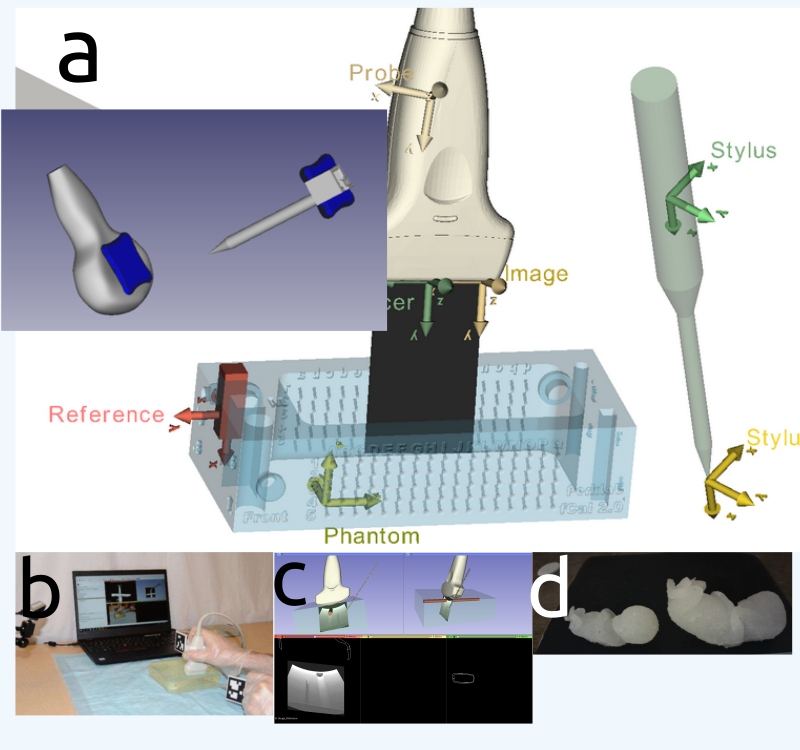
\includegraphics[width=0.9\textwidth]{./figures/sugi/plan-simulator-for-ugi/versions/drawing-v02.png}
%      \end{figure}
%
%    \end{column}
%  \end{columns}
%
%\end{frame}
%}
%%%%%%%%%%%%%%%%%%%%%%%%%%%%%%%%%%%%%%%%%%%%
\section{Conclusions and Future work}

%%%%%%%%%%%%%%%%%%%%%%%%%%%%%%%%%%%%%%%%%%%%%%%%%%%%%%%%
{
%\paper{Lastname N. YEAR in journal of...}
\begin{frame}{Conclusions and future work}

  \begin{columns}
  \begin{column}{.75\linewidth}

  \textbf{Conclusions}   

  We ....
  \begin{itemize}
    \item
  \end{itemize}

  \textbf{Future work}
  \begin{itemize}
    \item ...
    \item ...
  \end{itemize}

    \end{column}


  \begin{column}{.3\linewidth}

      \begin{figure}
        \centering
        %
\includegraphics[width=0.9\textwidth]{./figures/future-work/versions/drawing-v00.png}
      \end{figure}

    \end{column}
  \end{columns}

\end{frame}
}


%%%%%%%%%%%%%%%%%%%%%%%%%%%%%%%%%%%%%%%%%%%%%%%%%%%%%%%%
{
%\paper{Lastname N. YEAR in journal of...}
\begin{frame}{Acknowledgements}

  \begin{figure}
  \centering
  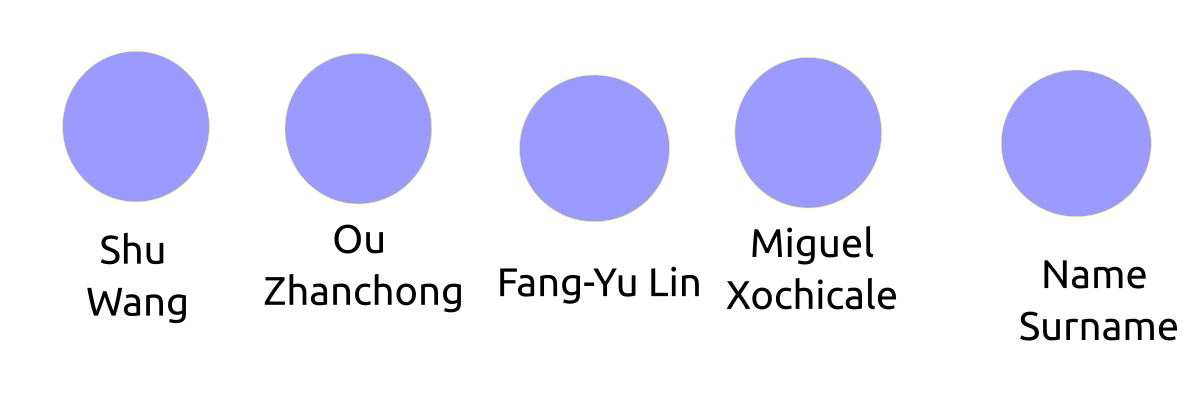
\includegraphics[width=1.0\textwidth]{./figures/team/versions/drawing-v01.png}
  \end{figure}

\end{frame}
}



%\begin{frame}[standout]
%  Thanks \\
%  Questions?
%\end{frame}

\maketitle

\end{document}
